Xác định số lượng cụm tối ưu trong một tập dữ liệu là vấn đề cơ bản trong phân cụm Kmeans, yêu cầu người dùng chỉ định số lượng cụm k được tạo. Ý tưởng đằng sau Kmeans bao gồm xác định các cụm k sao cho tổng biến thể trong cụm là tối thiểu. Đây được xem là một nhược điểm của thuật toán này. Phần dưới đây trình bày một vài phương pháp giúp xác định số cụm k hợp lý nhất.\par
\subsection{Thuật toán Elbow}
Tư tưởng chính của phương pháp phân cụm phân hoạch (như KMeans) là định nghĩa 1 cụm sao cho tổng bình phương khoảng cách của tất cả các điểm đến đến trung tâm cụm là nhỏ nhất, tham số này là WSS (Within-cluster Sum of Square). Elbow method chọn số cụm k sao cho khi thêm vào  một cụm khác thì không làm cho WSS thay đổi nhiều.\par
\smallskip
Quy trình triển khai thuật toán Elbow:
\begin{itemize}
	\item Thực hiện phân cụm với số cụm thay đổi
	\item Với mỗi giá trị k, tính giá trị WSS
	\item Vẽ đường cong Elbow theo các giá trị k
	\item Dựa vào đường cong Elbow chọn số k thích hợp, là vị trí ở khúc cua 
\end{itemize}
\newpage
Xét ví dụ mẫu dữ liệu sau:
\begin{figure}[h]
	\centering
	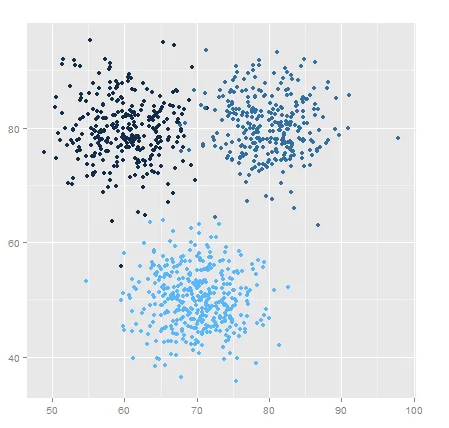
\includegraphics[width=0.5\linewidth]{img/data_set_1}
	\caption{Mẫu dữ liệu}
\end{figure}\par
Tính toán giá trị WSS tương ứng với K từ 1 đến 20, ta thu được biểu đồ sau:
\begin{figure}[h]
	\centering
	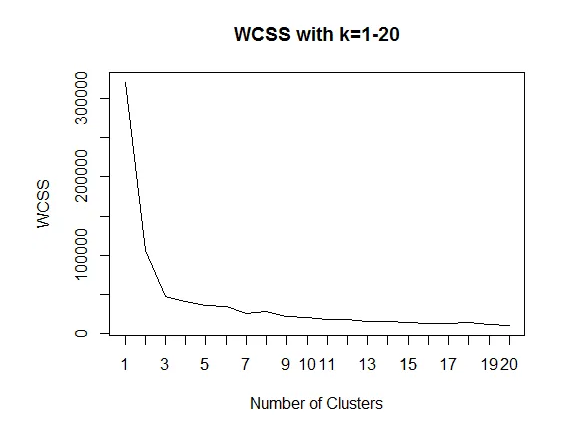
\includegraphics[width=0.6\linewidth]{img/data_set_2}
	\caption{WSS tương ứng với k từ 1 đến 20}
\end{figure}\par
Ta chọn k = 3 làm số cụm cho mẫu dữ liệu trên.
\newpage
\subsection{Thuật toán average silhouette}
Average silhouette dùng để đo chất lượng của một cụm. Giá trị Silhouette s(i) cho mỗi điểm dữ liệu i được xác định như sau:\\
\begin{center}
	\large
	$s(i) = \frac{b(i) - a(i)}{max\{a(i), b(i)\}} (|C_i| > 1)$
\end{center}\par
Trong đó:
\begin{itemize}
	\item a(i) khoảng cách trung bình từ điểm i đến các điểm khác trong cụm. $a(i) = \frac{1}{|C_i| - 1}\sum\limits_{j \in C_i, i \neq j}{d(i, j)}$
	\item b(i) là khoảng cách trung bình giữa các cụm. $b(i) = \underset{i \neq j}{min} \frac{1}{|C_j|}\sum\limits_{j \in C_j}{d(i, j)}$
\end{itemize}
Với s(i) = 0 với những cụm có chỉ có 1 phần tử.\par
\smallskip
Quy trình triển khai thuật toán average silhouette:
\begin{itemize}
	\item Thực hiện phân cụm với số cụm thay đổi
	\item Với mỗi giá trị k, tính giá trị average silhouette
	\item Vẽ đường cong average silhouette theo các giá trị k
	\item Vị trí có average silhouette lớn nhất là số cụm cần tìm
\end{itemize}
Xét ví dụ về mẫu dữ liệu sau:
\begin{figure}[h]
	\centering
	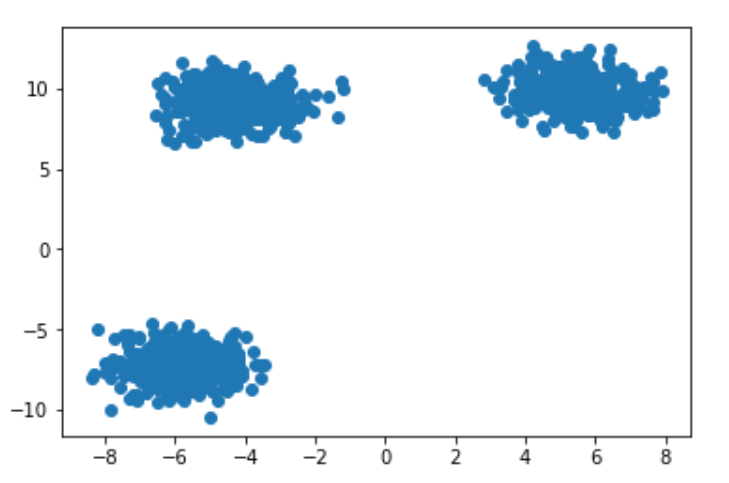
\includegraphics[width=0.5\linewidth]{img/data_set_3}
	\caption{Mẫu dữ liệu}
\end{figure}\par
Vẽ đường cong average silhouette:
\begin{figure}[h]
	\centering
	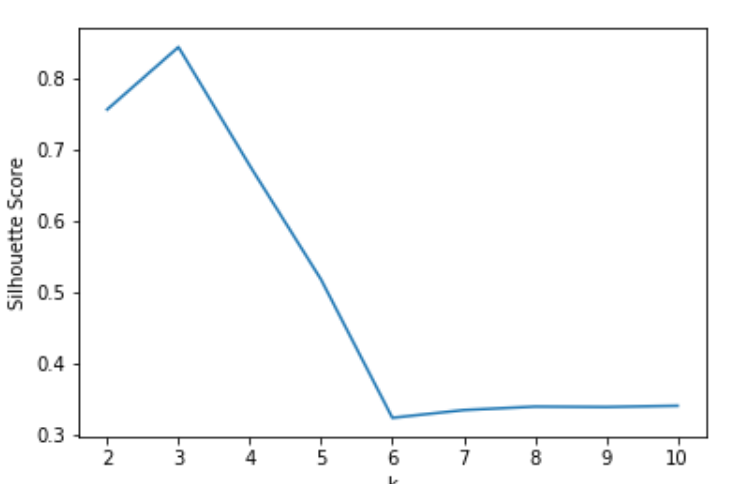
\includegraphics[width=0.5\linewidth]{img/data_set_4}
\end{figure}\par
Ta chọn k = 3 làm số cụm cho mẫu dữ liệu trên.